%%%%%%%%%%%%%%%%%%%%%%%%%%%%%%%%%%%%%%%%%
%  My documentation report
%  Objetive: Explain what I did and how, so someone can continue with the investigation
%
% Important note:
% Chapter heading images should have a 2:1 width:height ratio,
% e.g. 920px width and 460px height.
%
%%%%%%%%%%%%%%%%%%%%%%%%%%%%%%%%%%%%%%%%%


%----------------------------------------------------------------------------------------
%	PACKAGES AND OTHER DOCUMENT CONFIGURATIONS
%----------------------------------------------------------------------------------------

\documentclass[11pt,fleqn]{book} % Default font size and left-justified equations

\usepackage[top=3cm,bottom=3cm,left=3.2cm,right=3.2cm,headsep=10pt,letterpaper]{geometry} % Page margins

\usepackage{xcolor} % Required for specifying colors by name
\definecolor{ocre}{RGB}{52,177,201} % Define the orange color used for highlighting throughout the book

% Font Settings
\usepackage{avant} % Use the Avantgarde font for headings
%\usepackage{times} % Use the Times font for headings
\usepackage{mathptmx} % Use the Adobe Times Roman as the default text font together with math symbols from the Sym­bol, Chancery and Com­puter Modern fonts
\usepackage{microtype} % Slightly tweak font spacing for aesthetics
\usepackage[utf8]{inputenc} % Required for including letters with accents
\usepackage[T1]{fontenc} % Use 8-bit encoding that has 256 glyphs
\usepackage{amsthm}
\usepackage{algorithm}
\usepackage{algpseudocode}
% Bibliography
\usepackage[style=alphabetic,sorting=nyt,sortcites=true,autopunct=true,babel=hyphen,hyperref=true,abbreviate=false,backref=true,backend=biber]{biblatex}
\addbibresource{bibliography.bib} % BibTeX bibliography file
\defbibheading{bibempty}{}

%----------------------------------------------------------------------------------------
%	VARIOUS REQUIRED PACKAGES
%----------------------------------------------------------------------------------------

\usepackage{titlesec} % Allows customization of titles

\usepackage{graphicx} % Required for including pictures
\graphicspath{{Pictures/}} % Specifies the directory where pictures are stored
% \graphicspath{{Plots/}}
\usepackage{lipsum} % Inserts dummy text

\usepackage{tikz} % Required for drawing custom shapes

\usepackage[english]{babel} % English language/hyphenation

\usepackage{enumitem} % Customize lists
\setlist{nolistsep} % Reduce spacing between bullet points and numbered lists

\usepackage{booktabs} % Required for nicer horizontal rules in tables

\usepackage{eso-pic} % Required for specifying an image background in the title page

%----------------------------------------------------------------------------------------
%	MAIN TABLE OF CONTENTS
%----------------------------------------------------------------------------------------

\usepackage{titletoc} % Required for manipulating the table of contents

\contentsmargin{0cm} % Removes the default margin
% Chapter text styling
\titlecontents{chapter}[1.25cm] % Indentation
{\addvspace{15pt}\large\sffamily\bfseries} % Spacing and font options for chapters
{\color{ocre!60}\contentslabel[\Large\thecontentslabel]{1.25cm}\color{ocre}} % Chapter number
{}  
{\color{ocre!60}\normalsize\sffamily\bfseries\;\titlerule*[.5pc]{.}\;\thecontentspage} % Page number
% Section text styling
\titlecontents{section}[1.25cm] % Indentation
{\addvspace{5pt}\sffamily\bfseries} % Spacing and font options for sections
{\contentslabel[\thecontentslabel]{1.25cm}} % Section number
{}
{\sffamily\hfill\color{black}\thecontentspage} % Page number
[]
% Subsection text styling
\titlecontents{subsection}[1.25cm] % Indentation
{\addvspace{1pt}\sffamily\small} % Spacing and font options for subsections
{\contentslabel[\thecontentslabel]{1.25cm}} % Subsection number
{}
{\sffamily\;\titlerule*[.5pc]{.}\;\thecontentspage} % Page number
[] 

%----------------------------------------------------------------------------------------
%	MINI TABLE OF CONTENTS IN CHAPTER HEADS
%----------------------------------------------------------------------------------------

% Section text styling
\titlecontents{lsection}[0em] % Indendating
{\footnotesize\sffamily} % Font settings
{}
{}
{}

% Subsection text styling
\titlecontents{lsubsection}[.5em] % Indentation
{\normalfont\footnotesize\sffamily} % Font settings
{}
{}
{}
 
%----------------------------------------------------------------------------------------
%	PAGE HEADERS
%----------------------------------------------------------------------------------------

\usepackage{fancyhdr} % Required for header and footer configuration

\pagestyle{fancy}
\renewcommand{\chaptermark}[1]{\markboth{\sffamily\normalsize\bfseries\chaptername\ \thechapter.\ #1}{}} % Chapter text font settings
\renewcommand{\sectionmark}[1]{\markright{\sffamily\normalsize\thesection\hspace{5pt}#1}{}} % Section text font settings
\fancyhf{} \fancyhead[LE,RO]{\sffamily\normalsize\thepage} % Font setting for the page number in the header
\fancyhead[LO]{\rightmark} % Print the nearest section name on the left side of odd pages
\fancyhead[RE]{\leftmark} % Print the current chapter name on the right side of even pages
\renewcommand{\headrulewidth}{0.5pt} % Width of the rule under the header
\addtolength{\headheight}{2.5pt} % Increase the spacing around the header slightly
\renewcommand{\footrulewidth}{0pt} % Removes the rule in the footer
\fancypagestyle{plain}{\fancyhead{}\renewcommand{\headrulewidth}{0pt}} % Style for when a plain pagestyle is specified

% Removes the header from odd empty pages at the end of chapters
\makeatletter
\renewcommand{\cleardoublepage}{
\clearpage\ifodd\c@page\else
\hbox{}
\vspace*{\fill}
\thispagestyle{empty}
\newpage
\fi}

%----------------------------------------------------------------------------------------
%	THEOREM STYLES
%----------------------------------------------------------------------------------------

\usepackage{amsmath,amsfonts,amssymb,amsthm} % For math equations, theorems, symbols, etc

\newcommand{\intoo}[2]{\mathopen{]}#1\,;#2\mathclose{[}}
\newcommand{\ud}{\mathop{\mathrm{{}d}}\mathopen{}}
\newcommand{\intff}[2]{\mathopen{[}#1\,;#2\mathclose{]}}
\newtheorem{notation}{Notation}[chapter]

%%%%%%%%%%%%%%%%%%%%%%%%%%%%%%%%%%%%%%%%%%%%%%%%%%%%%%%%%%%%%%%%%%%%%%%%%%%
%%%%%%%%%%%%%%%%%%%% dedicated to boxed/framed environements %%%%%%%%%%%%%%
%%%%%%%%%%%%%%%%%%%%%%%%%%%%%%%%%%%%%%%%%%%%%%%%%%%%%%%%%%%%%%%%%%%%%%%%%%%
\newtheoremstyle{ocrenumbox}% % Theorem style name
{0pt}% Space above
{0pt}% Space below
{\normalfont}% % Body font
{}% Indent amount
{\small\bf\sffamily\color{ocre}}% % Theorem head font
{\;}% Punctuation after theorem head
{0.25em}% Space after theorem head
{\small\sffamily\color{ocre}\thmname{#1}\nobreakspace\thmnumber{\@ifnotempty{#1}{}\@upn{#2}}% Theorem text (e.g. Theorem 2.1)
\thmnote{\nobreakspace\the\thm@notefont\sffamily\bfseries\color{black}---\nobreakspace#3.}} % Optional theorem note
\renewcommand{\qedsymbol}{$\blacksquare$}% Optional qed square

\newtheoremstyle{blacknumex}% Theorem style name
{5pt}% Space above
{5pt}% Space below
{\normalfont}% Body font
{} % Indent amount
{\small\bf\sffamily}% Theorem head font
{\;}% Punctuation after theorem head
{0.25em}% Space after theorem head
{\small\sffamily{\tiny\ensuremath{\blacksquare}}\nobreakspace\thmname{#1}\nobreakspace\thmnumber{\@ifnotempty{#1}{}\@upn{#2}}% Theorem text (e.g. Theorem 2.1)
\thmnote{\nobreakspace\the\thm@notefont\sffamily\bfseries---\nobreakspace#3.}}% Optional theorem note

\newtheoremstyle{blacknumbox} % Theorem style name
{0pt}% Space above
{0pt}% Space below
{\normalfont}% Body font
{}% Indent amount
{\small\bf\sffamily}% Theorem head font
{\;}% Punctuation after theorem head
{0.25em}% Space after theorem head
{\small\sffamily\thmname{#1}\nobreakspace\thmnumber{\@ifnotempty{#1}{}\@upn{#2}}% Theorem text (e.g. Theorem 2.1)
\thmnote{\nobreakspace\the\thm@notefont\sffamily\bfseries---\nobreakspace#3.}}% Optional theorem note

%%%%%%%%%%%%%%%%%%%%%%%%%%%%%%%%%%%%%%%%%%%%%%%%%%%%%%%%%%%%%%%%%%%%%%%%%%%
%%%%%%%%%%%%% dedicated to non-boxed/non-framed environements %%%%%%%%%%%%%
%%%%%%%%%%%%%%%%%%%%%%%%%%%%%%%%%%%%%%%%%%%%%%%%%%%%%%%%%%%%%%%%%%%%%%%%%%%
\newtheoremstyle{ocrenum}% % Theorem style name
{5pt}% Space above
{5pt}% Space below
{\normalfont}% % Body font
{}% Indent amount
{\small\bf\sffamily\color{ocre}}% % Theorem head font
{\;}% Punctuation after theorem head
{0.25em}% Space after theorem head
{\small\sffamily\color{ocre}\thmname{#1}\nobreakspace\thmnumber{\@ifnotempty{#1}{}\@upn{#2}}% Theorem text (e.g. Theorem 2.1)
\thmnote{\nobreakspace\the\thm@notefont\sffamily\bfseries\color{black}---\nobreakspace#3.}} % Optional theorem note
\renewcommand{\qedsymbol}{$\blacksquare$}% Optional qed square
\makeatother

% Defines the theorem text style for each type of theorem to one of the three styles above
\newcounter{dummy} 
\numberwithin{dummy}{section}
\theoremstyle{ocrenumbox}


\newtheorem{theoremeT}[dummy]{Theorem}
\newtheorem{lemma}[dummy]{Lemma}
\newtheorem{observation}[dummy]{Observation}
\newtheorem{proposition}[dummy]{Proposition}
% \newtheorem{definition}[dummy]{Definition}
\newtheorem{claim}[dummy]{Claim}
\newtheorem{fact}[dummy]{Fact}
\newtheorem{assumption}[dummy]{Assumption}

\newtheorem{problem}{Problem}[chapter]
% \newtheorem{exercise}{Exercise}[chapter]
\theoremstyle{blacknumex}
\newtheorem{exampleT}{Example}[chapter]
\theoremstyle{blacknumbox}
\newtheorem{vocabulary}{Vocabulary}[chapter]
\newtheorem{definitionT}{Definition}[section]
\newtheorem{corollaryT}[dummy]{Corollary}
\theoremstyle{ocrenum}

%----------------------------------------------------------------------------------------
%	DEFINITION OF COLORED BOXES
%----------------------------------------------------------------------------------------

\RequirePackage[framemethod=default]{mdframed} % Required for creating the theorem, definition, exercise and corollary boxes

% Theorem box
\newmdenv[skipabove=7pt,
skipbelow=7pt,
backgroundcolor=black!5,
linecolor=ocre,
innerleftmargin=5pt,
innerrightmargin=5pt,
innertopmargin=5pt,
leftmargin=0cm,
rightmargin=0cm,
innerbottommargin=5pt]{tBox}

% Exercise box	  
\newmdenv[skipabove=7pt,
skipbelow=7pt,
rightline=false,
leftline=true,
topline=false,
bottomline=false,
backgroundcolor=ocre!10,
linecolor=ocre,
innerleftmargin=5pt,
innerrightmargin=5pt,
innertopmargin=5pt,
innerbottommargin=5pt,
leftmargin=0cm,
rightmargin=0cm,
linewidth=4pt]{eBox}	

% Definition box
\newmdenv[skipabove=7pt,
skipbelow=7pt,
rightline=false,
leftline=true,
topline=false,
bottomline=false,
linecolor=ocre,
innerleftmargin=5pt,
innerrightmargin=5pt,
innertopmargin=0pt,
leftmargin=0cm,
rightmargin=0cm,
linewidth=4pt,
innerbottommargin=0pt]{dBox}	

% Corollary box
\newmdenv[skipabove=7pt,
skipbelow=7pt,
rightline=false,
leftline=true,
topline=false,
bottomline=false,
linecolor=gray,
backgroundcolor=black!5,
innerleftmargin=5pt,
innerrightmargin=5pt,
innertopmargin=5pt,
leftmargin=0cm,
rightmargin=0cm,
linewidth=4pt,
innerbottommargin=5pt]{cBox}

% Creates an environment for each type of theorem and assigns it a theorem text style from the "Theorem Styles" section above and a colored box from above
\newenvironment{theorem}{\begin{tBox}\begin{theoremeT}}{\end{theoremeT}\end{tBox}}
\newenvironment{exercise}{\begin{eBox}\begin{exerciseT}}{\hfill{\color{ocre}\tiny\ensuremath{\blacksquare}}\end{exerciseT}\end{eBox}}				  
\newenvironment{definition}{\begin{dBox}\begin{definitionT}}{\end{definitionT}\end{dBox}}	
\newenvironment{example}{\begin{exampleT}}{\hfill{\tiny\ensuremath{\blacksquare}}\end{exampleT}}		
\newenvironment{corollary}{\begin{cBox}\begin{corollaryT}}{\end{corollaryT}\end{cBox}}	

%----------------------------------------------------------------------------------------
%	REMARK ENVIRONMENT
%----------------------------------------------------------------------------------------

\newenvironment{remark}{\par\vspace{10pt}\small % Vertical white space above the remark and smaller font size
\begin{list}{}{
\leftmargin=35pt % Indentation on the left
\rightmargin=25pt}\item\ignorespaces % Indentation on the right
\makebox[-2.5pt]{\begin{tikzpicture}[overlay]
\node[draw=ocre!60,line width=1pt,circle,fill=ocre!25,font=\sffamily\bfseries,inner sep=2pt,outer sep=0pt] at (-15pt,0pt){\textcolor{ocre}{R}};\end{tikzpicture}} % Orange R in a circle
\advance\baselineskip -1pt}{\end{list}\vskip5pt} % Tighter line spacing and white space after remark

%----------------------------------------------------------------------------------------
%	SECTION NUMBERING IN THE MARGIN
%----------------------------------------------------------------------------------------

\makeatletter
\renewcommand{\@seccntformat}[1]{\llap{\textcolor{ocre}{\csname the#1\endcsname}\hspace{1em}}}                    
\renewcommand{\section}{\@startsection{section}{1}{\z@}
{-4ex \@plus -1ex \@minus -.4ex}
{1ex \@plus.2ex }
{\normalfont\large\sffamily\bfseries}}
\renewcommand{\subsection}{\@startsection {subsection}{2}{\z@}
{-3ex \@plus -0.1ex \@minus -.4ex}
{0.5ex \@plus.2ex }
{\normalfont\sffamily\bfseries}}
\renewcommand{\subsubsection}{\@startsection {subsubsection}{3}{\z@}
{-2ex \@plus -0.1ex \@minus -.2ex}
{.2ex \@plus.2ex }
{\normalfont\small\sffamily\bfseries}}                        
\renewcommand\paragraph{\@startsection{paragraph}{4}{\z@}
{-2ex \@plus-.2ex \@minus .2ex}
{.1ex}
{\normalfont\small\sffamily\bfseries}}

%----------------------------------------------------------------------------------------
%	HYPERLINKS IN THE DOCUMENTS
%----------------------------------------------------------------------------------------

% For an unclear reason, the package should be loaded now and not later
\usepackage{hyperref}
\hypersetup{hidelinks,backref=true,pagebackref=true,hyperindex=true,colorlinks=false,breaklinks=true,urlcolor= ocre,bookmarks=true,bookmarksopen=false,pdftitle={Title},pdfauthor={Author}}

%----------------------------------------------------------------------------------------
%	CHAPTER HEADINGS
%----------------------------------------------------------------------------------------

% The set-up below should be (sadly) manually adapted to the overall margin page septup controlled by the geometry package loaded in the main.tex document. It is possible to implement below the dimensions used in the goemetry package (top,bottom,left,right)... TO BE DONE

\newcommand{\thechapterimage}{}
\newcommand{\chapterimage}[1]{\renewcommand{\thechapterimage}{#1}}

% Numbered chapters with mini tableofcontents
\def\thechapter{\arabic{chapter}}
\def\@makechapterhead#1{
\thispagestyle{empty}
{\centering \normalfont\sffamily
\ifnum \c@secnumdepth >\m@ne
\if@mainmatter
\startcontents
\begin{tikzpicture}[remember picture,overlay]
\node at (current page.north west)
{\begin{tikzpicture}[remember picture,overlay]
\node[anchor=north west,inner sep=0pt] at (0,0) {\includegraphics[width=\paperwidth]{\thechapterimage}};
%%%%%%%%%%%%%%%%%%%%%%%%%%%%%%%%%%%%%%%%%%%%%%%%%%%%%%%%%%%%%%%%%%%%%%%%%%%%%%%%%%%%%
% Commenting the 3 lines below removes the small contents box in the chapter heading
%\fill[color=ocre!10!white,opacity=.6] (1cm,0) rectangle (8cm,-7cm);
%\node[anchor=north west] at (1.1cm,.35cm) {\parbox[t][8cm][t]{6.5cm}{\huge\bfseries\flushleft \printcontents{l}{1}{\setcounter{tocdepth}{2}}}};
\draw[anchor=west] (5cm,-9cm) node [rounded corners=20pt,fill=ocre!10!white,text opacity=1,draw=ocre,draw opacity=1,line width=1.5pt,fill opacity=.6,inner sep=12pt]{\huge\sffamily\bfseries\textcolor{black}{\thechapter. #1\strut\makebox[22cm]{}}};
%%%%%%%%%%%%%%%%%%%%%%%%%%%%%%%%%%%%%%%%%%%%%%%%%%%%%%%%%%%%%%%%%%%%%%%%%%%%%%%%%%%%%
\end{tikzpicture}};
\end{tikzpicture}}
\par\vspace*{230\p@}
\fi
\fi}

% Unnumbered chapters without mini tableofcontents (could be added though) 
\def\@makeschapterhead#1{
\thispagestyle{empty}
{\centering \normalfont\sffamily
\ifnum \c@secnumdepth >\m@ne
\if@mainmatter
\begin{tikzpicture}[remember picture,overlay]
\node at (current page.north west)
{\begin{tikzpicture}[remember picture,overlay]
\node[anchor=north west,inner sep=0pt] at (0,0) {\includegraphics[width=\paperwidth]{\thechapterimage}};
\draw[anchor=west] (5cm,-9cm) node [rounded corners=20pt,fill=ocre!10!white,fill opacity=.6,inner sep=12pt,text opacity=1,draw=ocre,draw opacity=1,line width=1.5pt]{\huge\sffamily\bfseries\textcolor{black}{#1\strut\makebox[22cm]{}}};
\end{tikzpicture}};
\end{tikzpicture}}
\par\vspace*{230\p@}
\fi
\fi
}
\makeatother % Insert the commands.tex file which contains the majority of the structure behind the template

%----------------------------------------------------------------------------------------
%	Definitions of new commands
%----------------------------------------------------------------------------------------

\def\R{\mathbb{R}}
\newcommand{\cvx}{convex}
\begin{document}

%----------------------------------------------------------------------------------------
%	TITLE PAGE
%----------------------------------------------------------------------------------------

\begingroup
\thispagestyle{empty}
\AddToShipoutPicture*{\put(0,0){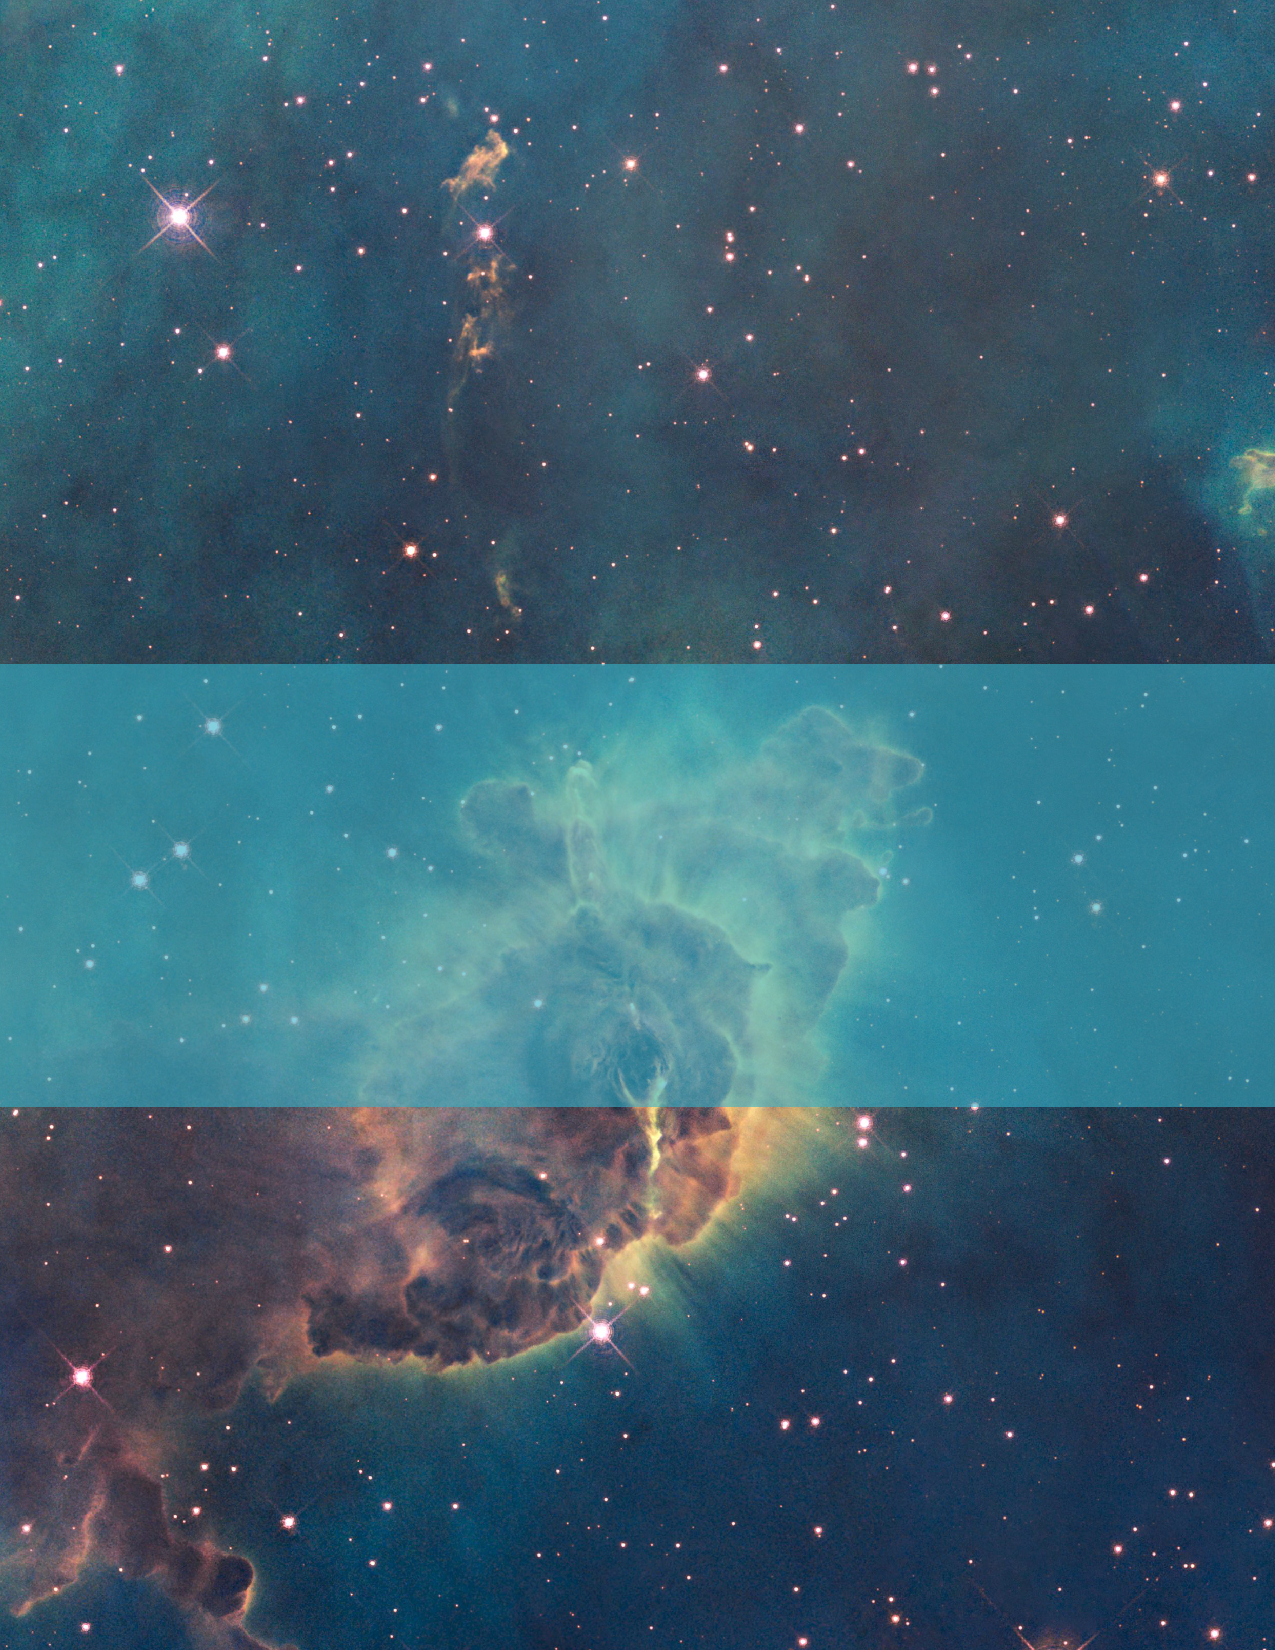
\includegraphics[scale=1.25]{esahubble}}} % Image background
\centering
\vspace*{5cm}
\par\normalfont\fontsize{35}{35}\sffamily\selectfont
\textbf{August, 2017}\\
{\LARGE Probability Ideas in Computing}\par % Book title
\vspace*{1cm}
{\Huge Lecture Notes}\par % Author name
\endgroup

%----------------------------------------------------------------------------------------
%	COPYRIGHT PAGE
%----------------------------------------------------------------------------------------

\newpage
~\vfill
\thispagestyle{empty}

%\noindent Copyright \copyright\ 2014 Andrea Hidalgo\\ % Copyright notice

\noindent \textsc{Indian Institute of Technology, Ropar}\\

\noindent \textsc{github.com/yytgpt/Probability-Ideas-in-Computing}\\ % URL

\noindent This book was written under the supervision of Dr. S.R.S. Iyengar \\ % License information

\noindent \textit{First release, December 2017} % Printing/edition date

%----------------------------------------------------------------------------------------
%	TABLE OF CONTENTS
%----------------------------------------------------------------------------------------

\chapterimage{head1.png} % Table of contents heading image

\pagestyle{empty} % No headers

\tableofcontents % Print the table of contents itself

%\cleardoublepage % Forces the first chapter to start on an odd page so it's on the right

\pagestyle{fancy} % Print headers again

%----------------------------------------------------------------------------------------
%	CHAPTER 1
%----------------------------------------------------------------------------------------

\chapterimage{monty.png} % Chapter heading image
\chapter{Lecture-1}
\section{The Monty Hall Show}

The Monty Hall problem is based on the American reality show - ``Let's make a deal'' and is named after its host, Monty Hall. \\

Before explaining the Monty Hall game, let us understand a simpler scenario. Assume you are the contestant of a reality show. On the stage, there are $3$ doors present in front of you. Out of these $3$ doors, $1$ door contains BMW car and rest of the two doors contain goats. You as a contestant do not know what is hidden inside these gates. You are asked to choose one gate and you get what is hidden inside the gate. Obviously, you are considered to win if and only if you choose the gate hiding the BMW car.  

In this simple scenario, probability of winning = $1/3$ and probability of losing = $2/3$.\\

\textbf{Now, we introduce the Monty Hall problem which brings in a twist to this simple scenario.}\\

Monty Hall is now the smart anchor of our show and enters the scene. He asks you to choose one door, similar to the previous case. You choose any one of the gates as in the previous case. But before declaring the result, Monty shows you the one gate hiding a goat out of the two gates which you have not chosen\footnote{Monty knows which door has what. That's why he is capable of opening a door which has a goat hidden.}. Since, there are two doors hiding goats, there is definitely at least one goat in the gates which you have not chosen. Now, you are given an option to swap your choice and choose the third gate which is unopened and previously not chosen by you. This has been shown in Figure \ref{monty} \\

\begin{figure}[h]
\centering
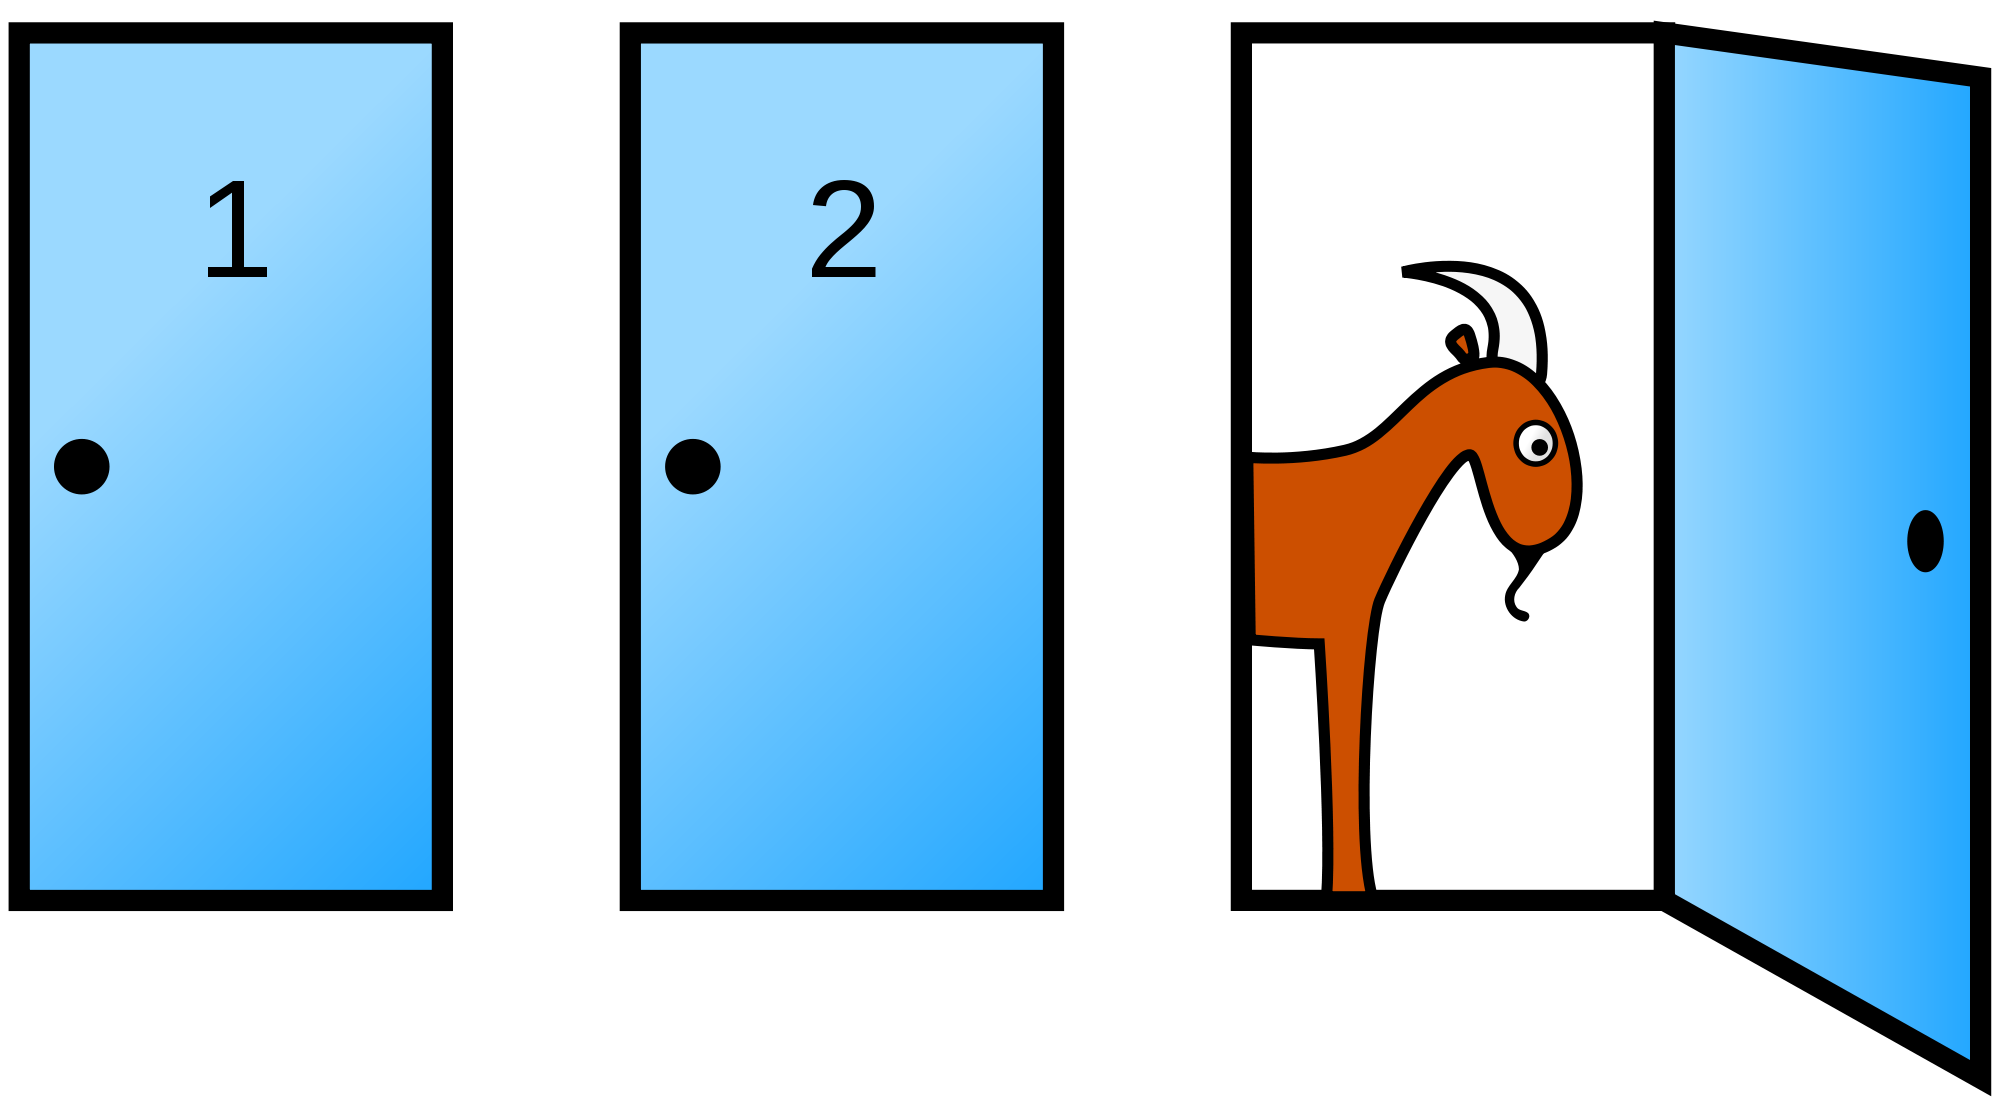
\includegraphics[width=0.5\textwidth]{monty.png}
\caption{The Monty Hall Game}
\label{monty}
\end{figure}

\textit{SHOULD YOU SWAP YOUR CHOICE AND GO WITH THIS THIRD GATE OR IT DOES NOT MATTER? Do you think swapping makes any difference to your probability of winning?}

Let us consider the two cases, one where you swap and the other where you do not swap. \\

\textbf{Case 1}:\textit{ You do not swap}: So, you have chosen one door and after knowing which of the other two doors has a goat, you do not swap your choice. So, this extra knowledge does not matter to your answer.
Hence, Probability (Win) = 1/3 and Probability (Losing) = 2/3

\textbf{Case 2:} \textit{You swap:}\\ 
\textit{Case 2.a :} You have initially chosen a door containing a goat.\\ 
Probability (You have chosen a door containing goat) = $2/3$. Now Monty shows you the other door having a goat. So, when you swap, you definitely pick the door having BMW. Hence, your probability of winning = $2/3$.\\

\textit{Case 2.b : }You have initially chosen the door containing BMW.\\ 
Probability (You have chosen the door containing BMW) = $1/3$. Now Monty shows you the other door having a goat. So, when you swap, you definitely pick the door having another goat. Hence, your probability of losing= $1/3$.\\

Hence, we see that swapping the gates results in the swapping of the probabilities of winning and losing thereby making win more likely. \\

\textbf{Case 3:} \textit{You swap with a probability $p$:}\\

Consider Figure \ref{modi}
\begin{figure}[h]
\centering
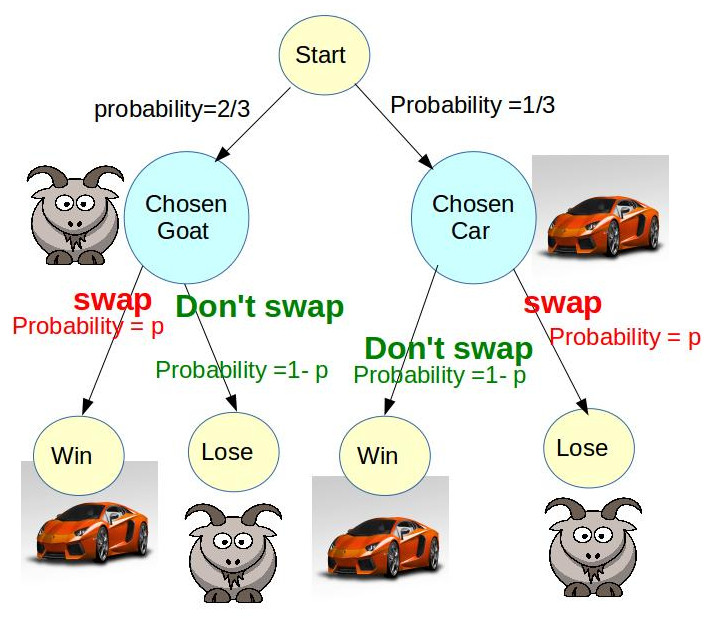
\includegraphics[width=\textwidth]{goat.jpg}
\caption{Modified Monty Hall Problem}
\label{modi}
\end{figure}

It can be seen that the player wins if she initially chooses goat and then swap, or initially chooses car and then do not swap.\\

Hence, the probability of winning = $\frac{2}{3} \times p\ +\ \frac{1}{3} \times (1-p)$\\

= $\frac{1}{3}p + \frac{1}{3}$\\

= $\frac{1+p}{3}$

Similarly, player loses if she initially chooses goat and do not swap or if she initially chooses car and then swap. \\

Hence, the probability of losing= $\frac{2}{3} \times (1-p)\ +\ \frac{1}{3} \times p$

= $\frac{2}{3} - \frac{1}{3}p$

= $\frac{2-p}{3}$ 

\section{The Coin Tossing Game}
\textbf{The Game}: In a contest, a participant tosses a coin. If the coin shows up tail, an amount of $100$ \$ is placed on the table in front of him, and he continues tossing. If the coin shows up a head, an amount of $100$ \$ is kept on the same table and then all the money kept on the table is given to the participant concluding the game. It can be seen that the participant wins a cash amount of $100 \times number\ of\ coins\ tossed$. \\

\textbf{Question:} What is the expected value of cash price won by the participant?\\

\textbf{Answer}: 
Let $X$ be a random variable which counts the number of times the coin is tossed.\\

We know that $X$ can take the values 1, 2, 3, 4.......\\
$E[X]\ =\ 1 \times pr(X=1) + 2 \times pr(X=2) + 3 \times pr(X=3)+ .... $\\

= $\sum_{i=1}^{\infty} i \times pr(X=i) $\\

Since, $ pr(X=i) $ = $(1/2)^i$\\

Hence, $E[X]\ = \sum_{i=1}^{\infty} i/2^{n} $\\

= $1/2+(2/2^2)+(3/2^3)+(4/2^4)+.....\ =\ \alpha$, say\\

Now, $\alpha = 1/2+(2/2^2)+(3/2^3)+(4/2^4)+.....$ \hspace{5mm} ........(1)\\

$\alpha/2 = (1/2^2)+(2/2^3)+(3/2^4)+.....$\hspace{5mm} ........(2)\\

Subtracting equation (2) from equation (1) \\

$\alpha/2= (1/2)+(1/2^2)+(1/2^3)+.....$\\

It can be seen that the above expression is a geometric progression $a,ar,ar^2,ar^3......$, with $a=1$ and $r=1/2$.\\

We know that the sum of an infinite Geometric Progression = $\frac{a}{1-r}$ = $\frac{1/2}{1-1/2}$ (in this case) = $1$. \\

Hence, $\alpha/2\ = 1$\\

$\alpha=2$\\

$E[X]=2$\\  	\hspace{5mm} ........(3)

So, the expected amount of money won by the participant = $2 \times 100$ \$ = $200$ \$.\\

Now, we know that the expected amount of money won by the participant is $200$ \$. But, the standard deviation of the amount of money won (or the number of coin tosses done) can be very large\footnote{When the game is actually played, the participant can win $100$ \$ in one case, yet $500$ \$ in other case, yet $10000$ \$ in other case.}. Hence, it is important to look at the standard deviation of the random variable $X$, in addition to its expected value.\\

The formula for Standard Deviation, $\sigma(X)$, is given as :\\ 

$\sigma(X)$= $ \sqrt{(E[X- \mu])^2} $, where $\mu = E[X]$\\


= $ \sqrt{E[X^2 - 2 X \mu + \mu ^ 2]} $\\

= $ \sqrt{E[X^2 ]- 2 E[X] \mu + E[\mu ^ 2]} $\\

= $ \sqrt{E[X^2 ]- 2 \mu^2 + \mu ^ 2} $\\

= $ \sqrt{E[X^2 ]- \mu ^ 2} $\\

= $ \sqrt{E[X^2 ]- (E[X]) ^ 2} $\\

Hence, $\sigma(X)$=  $ \sqrt{E[X^2 ]- (E[X]) ^ 2} $	(4)\\

$X^2$ is also a random variable, which takes the values $1^2, 2^2, 3^2, 4^2..........$\\

$Pr(X^2=1^2) = Pr(X=1) = 1/2$\\

$Pr(X^2=2^2) = Pr(X=2) = 1/2^2$\\

... and so on \\

According the the expectation formula, $E[X^2] = 1^2 \times \frac{1}{2} + 2^2 \times \frac{1}{2^2} + 3^2 \times \frac{1}{2^3} + ............  $ = $\alpha$ say\\

$\alpha\ =\ \frac{1^2}{2^1} + \frac{2^2}{2^2} + \frac{3^2}{2^3} + \frac{4^2}{2^4} + .... $   \hspace{5mm} ........(5) \\	


$\alpha/2\ =\ \frac{1^2}{2^2} + \frac{2^2}{2^3} + \frac{3^2}{2^4} + \frac{4^2}{2^5} + .... $   \hspace{5mm} ........(6)  \\

Subtracting equation (6) from equation (5)\\

$\alpha/2\ =\ \frac{1^2}{2^1} + \frac{2^2-1^2}{2^2} + \frac{3^2-2^2}{2^3} + \frac{4^2-3^2}{2^4} + .... $    \\


or, $\alpha/2\ =\ \frac{1^2}{2^1} + \frac{(2+1)(2-1)}{2^2} + \frac{(3+2)(3-2)}{2^3} + \frac{(4+3)(4-3)}{2^4} + .... $    \\


or, $\alpha/2\ =\ \frac{1}{2^1} + \frac{3}{2^2} + \frac{5}{2^3} + \frac{7}{2^4} + .... $     \hspace{5mm} ........(7)\\	

Dividing equation (7) by equation (2)\\

 or, $\alpha/4\ =\ \frac{1}{2^2} + \frac{3}{2^3} + \frac{5}{2^4} + \frac{7}{2^5} + .... $  \hspace{5mm} ........(8)\\
 
 Subtracting equation (8) from equation (7)\\
 
$\alpha/4\ =\ \frac{1}{2} + \frac{2}{2^2} + \frac{2}{2^3} + \frac{2}{2^4} + .... $\\

or, $\alpha/4\ =\ 1 + \frac{1}{2^2} + \frac{1}{2^3} + \frac{1}{2^4} + .. $\\ 

or, $\alpha/4\ =\frac{3}{2}$, (applying the formula for sum of Geometric Progression)\\

$\alpha = 6$, \\

$E[X^2]=6$	\hspace{5mm} ........(9)\\

Substituting equation (3) and equation (9) in equation (4), \\

$\sigma(X)$=  $ \sqrt{6- 2 ^ 2} $\\

= $\sqrt{2}$\\

	
\textbf{Brain Teasers}
\begin{enumerate}
\item State whether series is convergent $\sum_{n=1}^{\infty} n/2^{n} $
\item State whether the series is convergent $\sum_{n=1}^{\infty} 1/n$ 
\end{enumerate}










\chapter{The Online Hiring/Dating Problem}
\section{Some interesting math jokes and to be thought about questions}

{\footnotesize These paradoxes have not been discussed in detail in the class. They will be covered in the tutorial session.}

\begin{enumerate}

\item A mathematician was caught hiding a bomb in his bag while boarding onto the flight from England to Canada. When asked why he has done so, he says - ``The probability of a man carrying a bomb in a flight = $\frac{1}{1000}$, which is still very high. So I could not have my peace of mind on the journey. But the probability of two people carrying a bomb in the flight = $\frac{1}{1000} \times \frac{1}{1000}\ = \frac{1}{1000000}$, which is very less. So if I carry a bomb, the probability of another bomb being present in this flight reduces by a very big extent."\\
\textit{To think:}What is wrong about these reasoning. 

\item Imagine a very old building standing intact from millions of years. Let $P(today)$ = The probability that this building will fall today and $P(tomorrow)$ = The probability that this building will fall tomorrow. \\
\textit{To think}: Whether $P(today)<P(tomorrow)$, or $P(today)>P(tomorrow)$ or $P(today)=P(tomorrow)$ ?

\item Consider a multiple choice exam conducted countrywide. There are two students- $A$ and $B$. $A$ and $B$ both have got equal marks. But $A$ knew the answers correctly of the questions he answered, while $B$ answered the questions randomly and was lucky enough to get the same marks as $A$. \\
\textit{To think:} By looking at their OMR\footnote{Optical Mark Reading- One where we darken the bubbles corresponding to the correct answer- A/B/C/D.} sheets, can you tell, which is the sheet of $A$ and which is the sheet of $B$.

\end{enumerate}


\section{Online Hiring/ Dating Problem}
\textbf{Problem Statement}: You are searching for a match for marriage. There are $1000$ boys standing in a row, and you have to choose one out of them. According to the rules of the game, you can interview the boys only in a sequence one by one. If the sequence is : \\ $B_1\ B_2\ B_3\ B_4\ B_5\ ....... \ B_{1000}\ $, you will first see $B_i$, only then $B_{i+1}$. You have a choice to accept or reject a boy. If you accept one, the game gets over and you tie a knot with the selected individual. If you reject a boy, you can not return back to him. He is gone forever. What should be the optimal strategy to choose as best person as possible?  

\textbf{Solution:} \\
\textit{Intuition:} Check out on some people. This will give you an idea of what the crowd is like. After getting the idea of the crowd, it will be easier to choose the best person. \\

Look for the first $k$ boys. Let $B_k$ be the best among these. Reject all of these $k$ boys and keep a note of $B_k$. After k boys, as soon as you see a boy better than $B_k$, you accept. This has been shown in Figure \ref{boy}.

\begin{figure}[h]
\centering
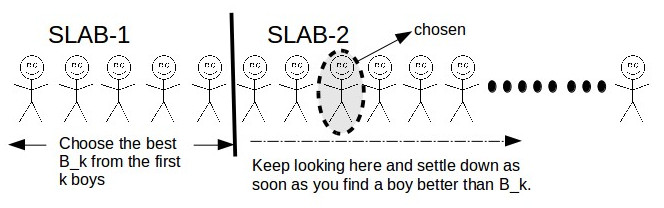
\includegraphics[width=0.9\textwidth]{boys.jpg}
\label{boy}
\caption{The technique to choose as best boy as possible}
\end{figure}

As an intelligent reader can make out, the value of $k$ plays a significant role here. If the value of $k$ is very small, you will end up choosing an inferior quality boy, since you have not seen enough samples. If $k$ is very big, not enough boys will be left in slab 2 to take a proper decision. So, now we look at the question - What should be the value of $k$.\\

Let $f(k)$ denote the quality of the selected boy when the first $k$ boys are employed as the sample of the entire population of available choices. We can plot a curve with $k$ on the X axis and $f(k)$ on the Y axis\footnote{Try writing a piece of code and observe how this plot looks like}. The roots of the equation $f'(k\ =0)$ give us the value of $k$ for which $f(k)$ is maximum, or in other words, we get the highest quality boy. This has been explained in detail in Algorithm \ref{dating}.

\begin{algorithm}
\caption{The Dating Algorithm}\label{dating}
\begin{algorithmic}[1]
\Procedure{Dating}{}
\State \textbf{Input}:- Array of the quality of $n$ boys $A[1,2,.....,n]$, $A[i]$ represents the quality of the $i_{th}$ boy, $k$
\State \textbf{Output}: $A[Best]$- The quality of the solution, $Best$- The index of the selected boy.
\State $Best\ = 0$
\For {$i\ =\ 1\ to\ k$}
\If {$A[Best] < A[i]$}
\State $Best \gets i $
\EndIf
\EndFor
\For {$i = k+1\ to\ n$}
\If {$A[Best] < A[i]$}
\State $Best \gets i$
\State break
\EndIf
\EndFor
\State return $Best$, $A[Best]$
\EndProcedure
\end{algorithmic}
\end{algorithm}

\subsection{Probability that Algorithm \ref{dating} fetches you the best boy}

The algorithm fails to fetch the best boy when one of the following two events occur.
\begin{itemize}
\item When the best boy is in the first $k$ boys(Our sample of the crowd). It is because, according to the algorithm the first $k$ boys are rejected and hence the best boy will also be rejected.  
\item When we pick a boy after the first $k$ boys and he is non-best. This is shown in Figure \ref{hero}. Here, we end up picking a suboptimal boy which is sandwiched between the $k+1_{th}$ location boy and the best boy. 
\end{itemize}

\begin{figure}[h]
\centering
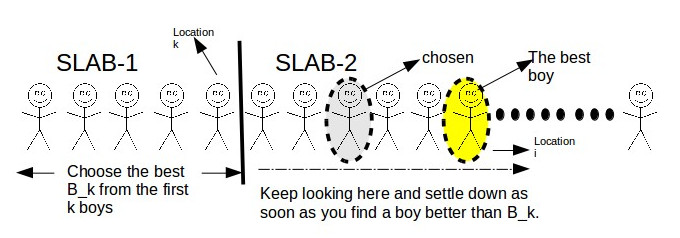
\includegraphics[width=0.9\textwidth]{hero.jpg}
\label{hero}
\caption{Choosing someone who is not the best}
\end{figure}

$Pr$(Best boy is in the first $k$ locations) = $ \frac{k}{n}$, since there are $k$ ways in which the best boy can be present at any of the first $k$ locations and the total number of locations to be present at are $n$. \\

We call a boy to be the pseudo-best if its quality is greater than $B_k$ and lesser than the quality of the best boy.
 
For the algorithm to fetch the best boy
\begin{enumerate}
\item The best boy should be present after the first $k$ locations. 
\item If the location of the best boy is $i$, no pseudo-best boy should be picked from the locations $[k+1,i-1]$.
\end{enumerate}


Hence, $Pr$(We get the best boy)= $Pr$(Best boy is at the location $i$ and no pseudo-best boy is present in the location $[k+1,i-1]$ ).\\

Given a location $i$, $Pr$(Best boy is present at this location) = $1/n$. \hspace{2mm} ....(1)\\

$Pr$(Pseudo-best boy is not there at locations $[k+1,i-1]$) = $\frac{k}{i-1}$. \hspace{2mm} ...(2) 

Why? Let us see.\\ 
We now, divide the queue of boys in three slabs as shown in Figure \ref{slabs}.

\begin{figure}[h]
\centering
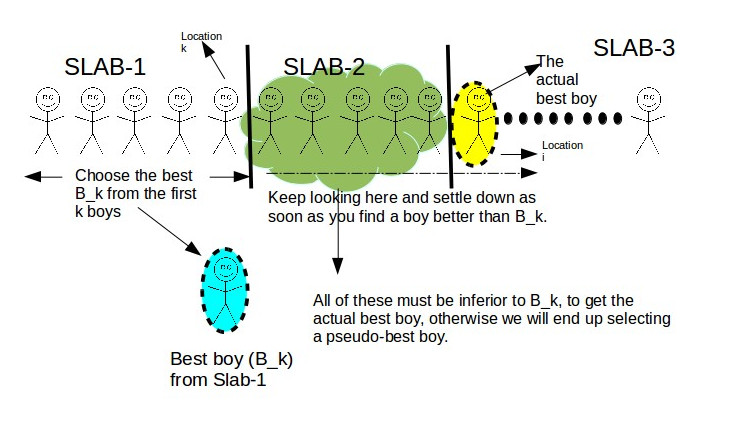
\includegraphics[width=0.9\textwidth]{slabs.jpg}
\label{slabs}
\caption{Choosing the best}
\end{figure}

$Pr$(The best boy from locations $1$ to $i-1$ is present before the location $k+1$)= $\frac{k}{i-1}$

From (1) and (2), \\
$pr$(winning when the best boy is at the location $i$) = $\frac{1}{n} \times \frac{k}{i-1}$\\

Now the location of the best boy can vary from $k+1$ to $n$. We have to take all these cases in account. \\

$Pr$(We end up choosing the best boy)= $\sum_{i=k+1}^n \frac{1}{n} \times \frac{k}{i-1}$\\

= $\frac{k}{n} \sum_{i=k+1}^n \frac{1}{i-1}$\\

= $\frac{k}{n} \sum_{i=k}^{n-1} \frac{1}{i}$\\

= $\frac{k}{n} \int_{k}^{n} \frac{1}{i} di$ (we replaced $n-1$ by $n$ assuming $n$ is a very large number)\\

= $\frac{k}{n}|log\ i|_{k}^{n}$\\

=$\frac{k}{n} (log\ n - log\ k)$\\

\[
 \boxed{f(k)\ =\ \frac{k}{n} (log\ n - log\ k)}
 \]
 
 Differentiating \\
 
 $f'(k)=\ \frac{1}{n} (log\ n\ -\ log\ k) + \frac{k}{n} \times \frac{-1}{k}$\\
 
 Equate to $0$. \\
 
 $\frac{1}{n} (log\ n\ -\ log\ k) + \frac{k}{n} \times \frac{-1}{k}\ =0$\\
 
 $ (log\ n\ -\ log\ k\ -\ 1\ = 0)$\\
 
 or, $log\ n\ -\ log_e\ e\ =\ log\ k$\\
 
 or, $log\ \frac{n}{e}\ =\ log\ k$\\
 
 or, 
\[
 \boxed{k=\ \frac{n}{e}}
 \]





\end{document}